%!TEX root = ../report.tex

\chapter{Stereovision} % (fold)
\label{chap:stereopsis}

\section{Introduction}
In this section, the solution adopted for the location of the target in the 3D space through the vision system, the reasons that led to this approach, the assumptions made and the obtained results are presented. 
A more detailed explanation of the 2D image processing performed for the target tracking can be found in \ref{chap:feature_extraction}.

\section{Stereopsis}
Due to the fact that two vision systems were available on the setup, the first step was to decide which one to employ and the method to compute disparity. 
After a slight evaluation of resources the chosen one was the stereo rig, utilized to carry out sparse stereo with a single well-defined point. 
Thus, the next points contain the steps to compute the position of a point in 3-space given its image in two views and the camera matrices. 

Through the acquired pairs of images, the pixel coordinates of the center of gravity of the target are extracted by the algorithm presented in \ref{chap:feature_extraction}, this has not been the approach adopted here.  and they are used to calculate its 3D coordinates referred to the camera reference frame by means of linear triangulation methods.

\section{Camera model}
As a consequence of the need of a defined relation between the image and the object space, the cameras must be used as a mapping. 
The mathematical model assumed for the camera is the basic pinhole structure, described in \cite{Hartley}. 
This model defines a linear projection from the 3D world to the image plane, and contains the intrinsic parameters that relates the camera and the image reference frames as showed in equation \ref{eq:pinhole_model}. Where X represent the homogeneous coordinates of a 3D point and x its projection in the image plane in pixel coordinates.
 
\begin{equation}
x = P·X
\label{eq:pinhole_model}
\end{equation}  

Since the linearity assumed by this model does not hold due to imperfections in the lens, a distortion model needs to be added to the calculations in order to correct the deviations on the real cameras. 
The Plumb Bob distortion model, introduced in \cite{Brown} is applied here since it is the one used by ROS.

\subsection{Calibration}
In order to obtain the intrinsic parameters for the camera model, a stereo calibration process based on the technique presented in \cite{Zhang} has been carried out for both Bumblebee2 1394a cameras by means of a ROS node. 

The node only needs to be provided enough images of a 2D calibration pattern in different positions. 
It computes the projection of the points on the pattern and solves the resulting equations system in a least squares fashion as described in ****reference(). 
The output of the node are the camera and projection matrices of the cameras, the set of parameters for the distortion model and the homography for the image rectification. 
Since the projection matrices will be used for the computation of the fundamental matrix during the triangulation calculus, their quality will heavily influence on the overall performance of the system. 
Therefore, a special commitment has been applied to this step. 

\section{Reconstruction of depth}
At this point the algorithm computes the camera matrices and the correspondent image points {xi, xi'} for two given images of the target. 
This information can be utilized to calculate depth by means of the disparity or difference in the x values of the image coordinates {xi, xi'}.

\begin{figure}[h]
    \centering
    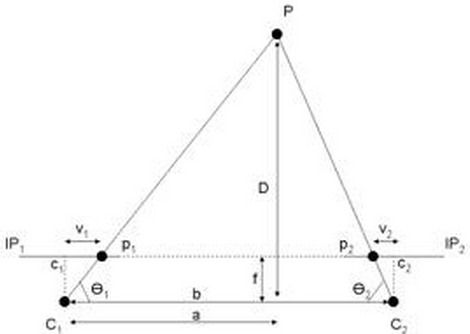
\includegraphics[width=0.5\textwidth]{images/triangulate}
    \caption{Depth measurement based on disparity}
    \label{fig:Depth_disparity}
\end{figure}

The stereovision system showed in \ref{fig:Depth_disparity}, equivalent to the employed in the project, is configured such that the optical axes of the cameras are parallel. 
This configuration yields horizontal epipolar lines and thus, eases the epipolar geometry resolution for this setup and could reduce the correspondence problem from two to one dimensions. However, as explained in \ref{chap:feature_extraction}, this has not been the approach adopted here. 

Once the disparity has been extracted, it can be used to calculate the XYZ coordinates of a 3D points solving Thale's theorem for the resulting triangles in the image as showed in \ref{eq:depth_meas} 

\begin{equation}
	X = XB/d $$
	Y = YB/d $$
	Z = Zf/d 	
	\label{eq:depth_meas}
\end{equation}  

The outputs from \ref{eq:depth_meas}, however, need to be adapted to the image reference frame. 

\section{Triangulation}
The next step is to define a suitable triangulation method light but robust enough to be executed in live with sufficient accuracy, since the whole system will rely on this task. 
An immediate, simple approach could consists in back-projecting the correspondent image points, by means of the projection matrix, and find the point in the space in which the intersect. However, due to the acquisition errors in the measured image coordinates, this procedure is very unlikely to succeed. 

\begin{figure}[h]
    \centering
   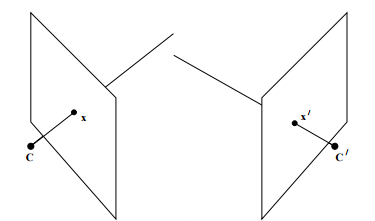
\includegraphics[width=0.8\textwidth]{figures/back_projection}
    \caption{Back-Projection rays error}
    \label{fig:Back-Projection}
\end{figure}

This is because in most of the cases the rays will not intersect in the 3D point, since there is not a point X that satisfies the equations \ref{eq:projection}. 

\begin{equation}
	\centering
	x  = P·X  $$\\
	x' = P·X' $$
	\label{eq:projection}
\end{equation} 


 









% section stereopsis (end)
  